\documentclass{article}

\usepackage{booktabs}
\usepackage{tabularx}
\usepackage{graphicx}
\usepackage{hyperref}
\usepackage{enumitem}
\usepackage[capitalise]{cleveref}

\input{../Comments}
\input{../Common}

\title{User Guide\\\progname{} (InfraRAT Web Application)}
\author{\authname}
\date{}

\begin{document}

\begin{table}[hp]
\caption{Revision History} \label{TblRevisionHistory}
\begin{tabularx}{\textwidth}{llX}
\toprule
\textbf{Date} & \textbf{Developer(s)} & \textbf{Change}\\
\midrule
2026-04-05 & Jeremy Orr & Initial user guide\\
2026-04-05 & --- & Restructured around user workflows; matches app navigation order\\
2026-04-05 & --- & Added per-area overviews (Home through About) before workflows\\
\bottomrule
\end{tabularx}
\end{table}

\vspace{0.5em}
\noindent\textit{Maintainers: add a row when user-visible behaviour changes.}

\newpage

\maketitle

\tableofcontents
\newpage

% ---------------------------------------------------------------------------
\section{How to use this guide}
\label{sec:how-to-use}

This guide is written for \textbf{you}---someone using InfraRAT in a web browser. You do not need technical setup.

\begin{itemize}[nosep]
  \item Read \cref{sec:map} for a short menu map, then \cref{sec:area-overview} if you want a fuller picture of what each screen contains.
  \item Skip to any \textbf{workflow} in \cref{sec:workflows} that matches what you want to do today. Each workflow is a numbered checklist you can follow in order.
  \item Use \cref{sec:reference} for file types, short definitions, and fixes when something blocks you.
\end{itemize}

\section{Introduction}
\label{sec:introduction}

The web application is branded \textbf{InfraRAT}. It supports data analysis for animal models of OCD on a large rat behavioural dataset (on the order of twenty thousand trials): natural-language questioning, tabular query results, inventory counts and session lists, charts and heatmaps, pre-built comparison dashboards, and per-session trajectory inspection.

This document explains what you see in the app and how to complete common tasks step by step. The product name in the header and footer is InfraRAT; \progname{} is the capstone project name on the title page.

\section{Quick start}
\label{sec:quick-start}

\begin{enumerate}[nosep]
  \item Open the web address your administrator gave you.
  \item Read \textbf{Home} for an overview, carousel cards, and example query wording.
  \item On \textbf{Query}, use \textbf{Ask} for conversational answers, or \textbf{Select} for tables and (when applicable) downloads.
  \item Open \textbf{Inventory} (\emph{Data Inventory}) to count sessions and files, optionally list up to 500 sessions, and download bundles.
  \item Use \textbf{Visualizations} for bar chart, heatmap, spatial heatmap, velocity profile, or \textbf{Query Visualizations}.
  \item Use \textbf{ToolBox} to load one session, inspect tables and the path view, and read summary metrics.
  \item Open \textbf{About} (info icon in the header) for team information and FAQs.
\end{enumerate}

\section{What is InfraRAT?}
\label{sec:what}

\textbf{InfraRAT} helps you explore a large rat behavioural dataset (tens of thousands of trials). In plain terms you can: ask questions, filter and count sessions, open charts and maps, compare groups on standard measures, inspect one session closely, and download selected file types for the sessions you care about.

The course project name is \progname{}; \textbf{InfraRAT} is the name in the app header.

\section{How the site is organized}
\label{sec:map}

The top bar matches the order below (on a phone, open the menu icon first). This is the same order as the workflows in the next section.

\begin{description}[style=nextline, font=\normalfont\bfseries]
  \item[Home] Orientation: what the platform does, rotating cards, and example wording (start here on day one).
  \item[Query] Ask questions in chat, or switch to Select to get tables and optional downloads (\emph{Talk to the FRDR}).
  \item[Visualizations] Pick a tool from the gallery (bar chart, heatmap, maps, velocity, dashboards).
  \item[Inventory] \emph{Data Inventory}---counts and filters across the dataset; list sessions and download bundles.
  \item[ToolBox] \emph{Analysis Toolbox}---one session at a time: tables, path view, summary numbers.
\end{description}

To the right: \textbf{About} (info icon) for team and FAQs; \textbf{GitHub} for reporting issues. The footer links to FRDR and the lab collection.

\textbf{Tip:} many tasks use two areas---for example Inventory to find IDs, then ToolBox or Visualizations to go deeper.

\section{Access and environment}
\label{sec:before}

There is no login or single sign-on screen in the current app: you use the deployment URL you were given.

If the header shows a \textbf{STAGING} badge next to the product name (for example when the app is run on a staging port), treat that environment as non-final.

\section{Overview of each area}
\label{sec:area-overview}

The subsections below describe \emph{what each part of the app is for} and what you will see there. Step-by-step instructions are in \cref{sec:workflows}.

\subsection{Header, footer, and navigation}
\label{subsec:layout-overview}

The header stays visible as you scroll. It shows the InfraRAT logo and name. The main destinations are \textbf{Home}, \textbf{Query}, \textbf{Visualizations}, \textbf{Inventory}, and \textbf{ToolBox}. On a narrow screen, open the menu control to reach the same links.

On the right, the \textbf{About} control (info icon) opens the About page. The \textbf{GitHub} icon opens the project issue tracker in a new tab (for feedback or bug reports).

The footer shows the app version (e.g.\ InfraRAT v1.0), course attribution, and links to FRDR and the Szechtman lab collection. If you open a bad link inside the app, you may see a simple ``not found'' page.

\subsection{Home}
\label{subsec:home-overview}

\textbf{Home} introduces the platform: purpose, scale (twenty-thousand-plus trials), and the idea of going from raw trials to insights.

An auto-advancing \textbf{carousel} presents use cases---dataset access and download, visualization and analysis, natural language questions, experiment playback, processing pipeline, and API-related messaging. These are overview cards, not separate apps.

Lower on the page, images contrast video trials with temporal or tabular views. Example natural-language prompts appear in quotation marks. A \textbf{sample results table} (trial ID, group, checking count, home-base duration, video sync, etc.) shows the \emph{shape} of tabular output; it is demo content, not live results from your run.

\subsection{Query}
\label{subsec:query-overview}

\textbf{Query} is the main chat-style interface to the dataset. The page title is \emph{Query}; the subtitle is \emph{Talk to the FRDR} (FRDR is the Federated Research Data Repository, also referenced when you download bundled files).

A switch toggles \textbf{Ask} and \textbf{Select}. In \textbf{Ask}, you type in everyday language and read a streamed answer in chat bubbles; emphasized phrases may appear in bold. In \textbf{Select}, the same kind of input produces a structured reply: \emph{Query Plan}, \emph{SQL Query}, and \emph{Results}. The embedded results table shows up to fifty rows, with a note if there are more.

Your messages appear on the right; the system's replies appear on the left.

Use the bottom text area (placeholder \emph{Ask, Search or Chat\ldots}). Press \textbf{Enter} to send and \textbf{Shift+Enter} for a new line without sending.

After a successful \textbf{Select} answer, a \textbf{Sessions} section below lists the full result set in a wide, scrollable table.

\textbf{Download Session Files} appears on this page only when the last message in the thread is a \textbf{Select} result (not a plain \textbf{Ask} reply). The dialog offers CSV, EWB, GIF, JPG, and MPG; after you confirm, a progress bar runs and your browser saves a ZIP whose name begins with \texttt{FRDR\_FILES\_}.

\subsection{Data Inventory}
\label{subsec:inventory-overview}

\textbf{Inventory} opens the \emph{Data Inventory} page. It explains that counts are by raw data type (video, track files, and related types) and that filters narrow which sessions are included.

\textbf{Show full inventory} and \textbf{Unoperated rats only} are shortcuts at the top. The left sidebar holds expandable filter groups: drug treatment (you may check several), file types, fine-grained drug regimens (labelled \emph{Drug Regiments} in the app), brain manipulation (surgery type and region), apparatus (including pattern and room), and session type. \textbf{Apply} runs the search; \textbf{Clear} resets choices and clears results and the session table.

After counts load, the main area shows how many sessions match, per-type file and session counts (with info tooltips), and a \textbf{Counts by data type} bar chart. \textbf{View sessions (up to 500)} loads a scrollable session table. \textbf{Download Session Files} in the sidebar is for the filtered list: it becomes available only after you have loaded that table and it is not empty. Format choices match the Query download dialog.

\subsection{Visualizations}
\label{subsec:viz-overview}

\textbf{Visualizations} opens a \textbf{gallery} of tiles. Each tile has a short description and an \textbf{Open} button. The gallery includes \textbf{Bar Chart}, \textbf{Heatmap}, \textbf{Spatial Heatmap}, \textbf{Velocity Profile}, and \textbf{Query Visualizations}. There is no tile for \textbf{Line Chart} on the gallery; that builder still exists in the app---ask your administrator for a bookmark or link if you need trends over time.

\textbf{Bar chart builder:} choose \textbf{X-Axis (Group By)} and \textbf{Y-Axis}; axis titles and units come from the data service.

\textbf{Line chart builder} (when you have a link): choose \textbf{X-Axis (Time Period)} and a \textbf{Y-Axis} metric for trends over time.

\textbf{Heatmap builder:} choose two dimensions and a \textbf{metric} for cell colour.

\textbf{Spatial heatmap:} combine one or more sessions, bin size, visits vs time in bin, optional fixed colour cap, optional \textbf{home base} rectangle, hover details on the map, and export to CSV or PNG.

\textbf{Velocity profile:} pick a session, define a circular zone (centre and radius), set frame windows and minimum trip length, choose colouring mode, then \textbf{Generate} to see entering and exiting speed traces.

\textbf{Query Visualizations:} choose a \textbf{Graph Set} (e.g.\ Tucci-style snapshot bars or Ballester-style lines across injections). Panels cover measures such as checking frequency, check length, recurrence time, stops before returning, and rest duration. Long on-page text describes the comparison design. Partial failures show a warning while other panels may still load.

\subsection{Analysis ToolBox}
\label{subsec:toolbox-overview}

\textbf{ToolBox} shows the \emph{Analysis Toolbox} page. Everything here is about \textbf{one session at a time}.

You search or pick a session ID, then \textbf{Load Session}. On success you typically see \textbf{Session Info} (metadata), \textbf{Data Points} (trajectory or frame table), a still \textbf{image} when available, and an \textbf{interactive path} plot of movement.

Three cards summarize \textbf{Distance Travelled} (metres), \textbf{Total Number of Checks}, and \textbf{Average Check Time} (shown as log$_{10}$ seconds). If distance is not available, \textbf{Generate Distance?} tries to compute it from identifiers in session info.

If the session cannot be loaded, the app states that it is not supported.

\subsection{About}
\label{subsec:about-overview}

\textbf{About} lists faculty and student contributors and credits a prior capstone team. An accordion holds FAQs (purpose, who can use the platform, what data exists, downloads). A button can take you to \textbf{Query} if you want to ask a follow-up question.

\subsection{Downloads and file formats (summary)}
\label{subsec:downloads-overview}

ZIP bundles from \textbf{Query} (after \textbf{Select}) and \textbf{Inventory} (after loading the session list) can include CSV, EWB, JPG, MPG, and GIF as you select them. Spatial heatmap exports use separate CSV/PNG actions on that page. Full detail is in \cref{ref:zip}.

\section{Guided workflows}
\label{sec:workflows}

Each workflow below is meant to be followed top to bottom. Screen names and button labels match the app.

\subsection{Workflow A: First visit---orient yourself}
\label{wf:orient}

\begin{enumerate}
  \item Open \textbf{Home}. Read the headline and short description of scale.
  \item Watch the \textbf{carousel}; each card states a capability (access, visualization, natural language, and so on).
  \item Skim the example questions and the \textbf{sample table}. The table is illustrative only---it shows the \emph{shape} of results, not live data.
  \item When you are ready to try the app, go to Workflow B or C.
\end{enumerate}

\begin{figure}[ht]
\centering
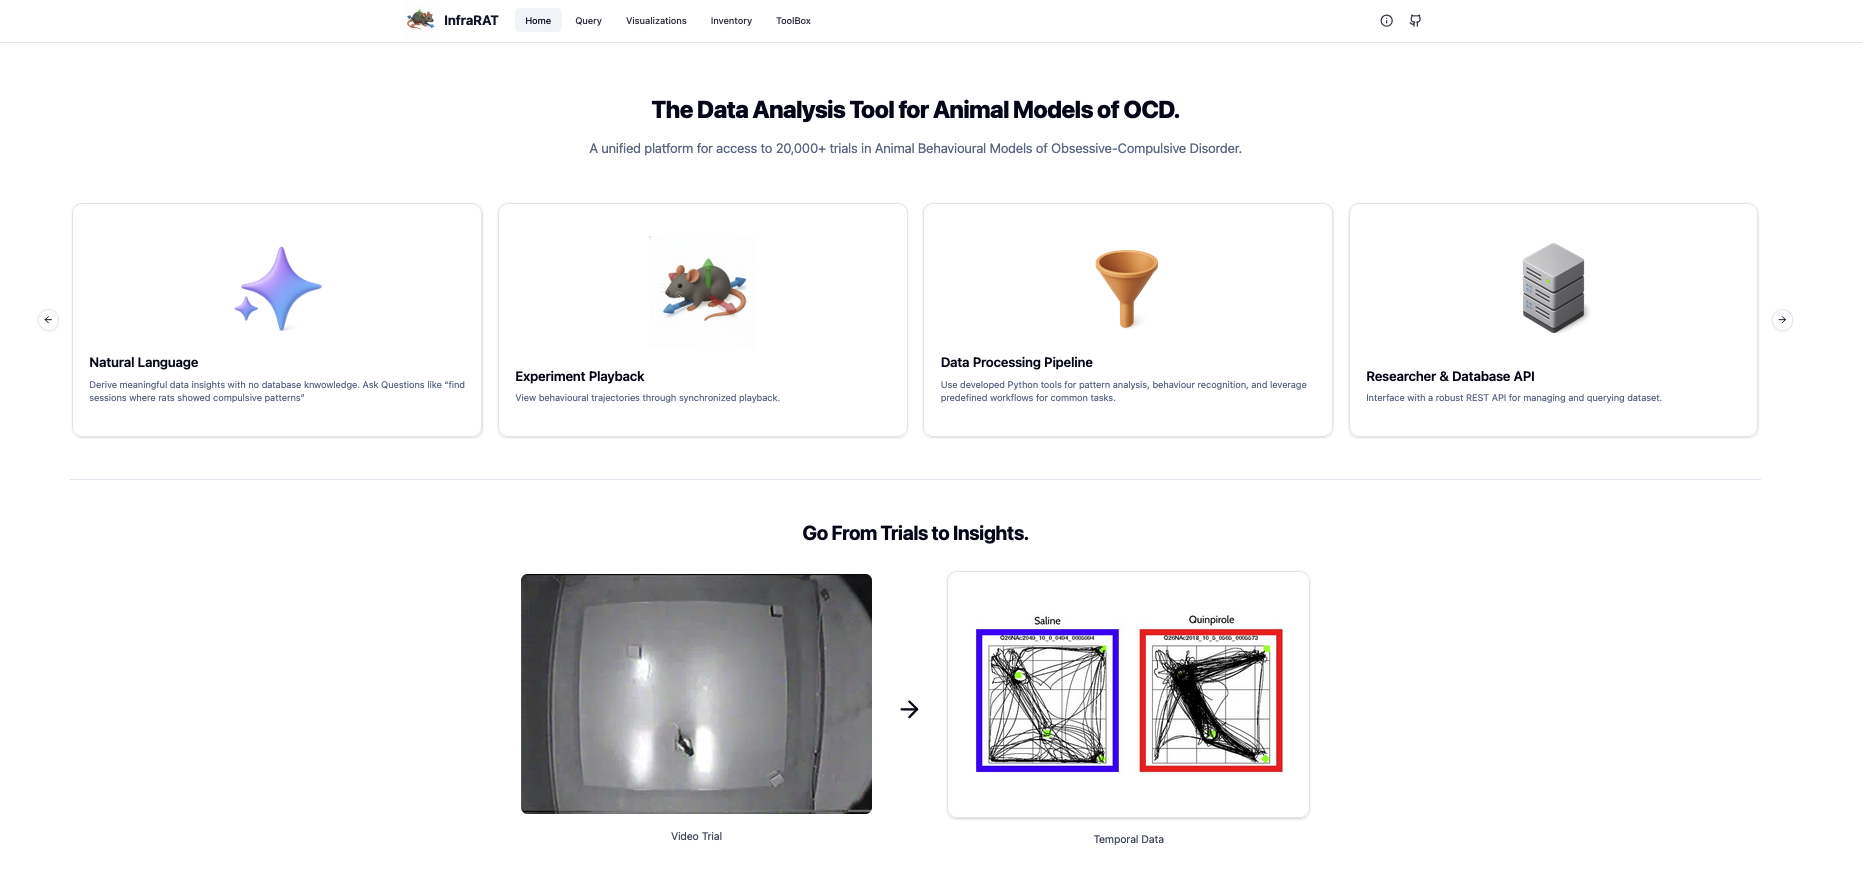
\includegraphics[width=0.95\textwidth]{homepage.png}
\caption{Home: start here to understand what InfraRAT offers.}
\label{fig:home}
\end{figure}

\subsection{Workflow B: Ask a question (no tables or downloads)}
\label{wf:ask}

\begin{enumerate}
  \item Click \textbf{Query} in the top bar.
  \item Leave the switch on \textbf{Ask} (left side).
  \item Type in the box at the bottom (``Ask, Search or Chat\ldots''). Press \textbf{Enter} to send, or \textbf{Shift+Enter} for a new line.
  \item Read the answer as it appears on the left. Important phrases may appear in \textbf{bold}.
\end{enumerate}

Use this when you want an explanation or exploration, not a spreadsheet or ZIP file.

\subsection{Workflow C: Get a table of sessions from a question (and optionally download)}
\label{wf:query-select}

\begin{enumerate}
  \item Go to \textbf{Query}. Flip the switch to \textbf{Select}.
  \item Type what you want in plain language; press \textbf{Enter} (or use the send button).
  \item On the left, read the card: \emph{Query Plan}, then \emph{SQL Query}, then \emph{Results}. The small table shows up to fifty rows; a note appears if there are more.
  \item Scroll down to \textbf{Sessions} to see the full table for that answer (wide columns---scroll sideways if needed).
  \item To download files for those sessions: click \textbf{Download Session Files}. It is enabled only if the \textbf{last} message in the thread is a Select result (not Ask). Choose CSV, EWB, GIF, JPG, and/or MPG, confirm, wait for the progress bar, then save the ZIP (name begins with \texttt{FRDR\_FILES\_}).
\end{enumerate}

\begin{figure}[ht]
\centering
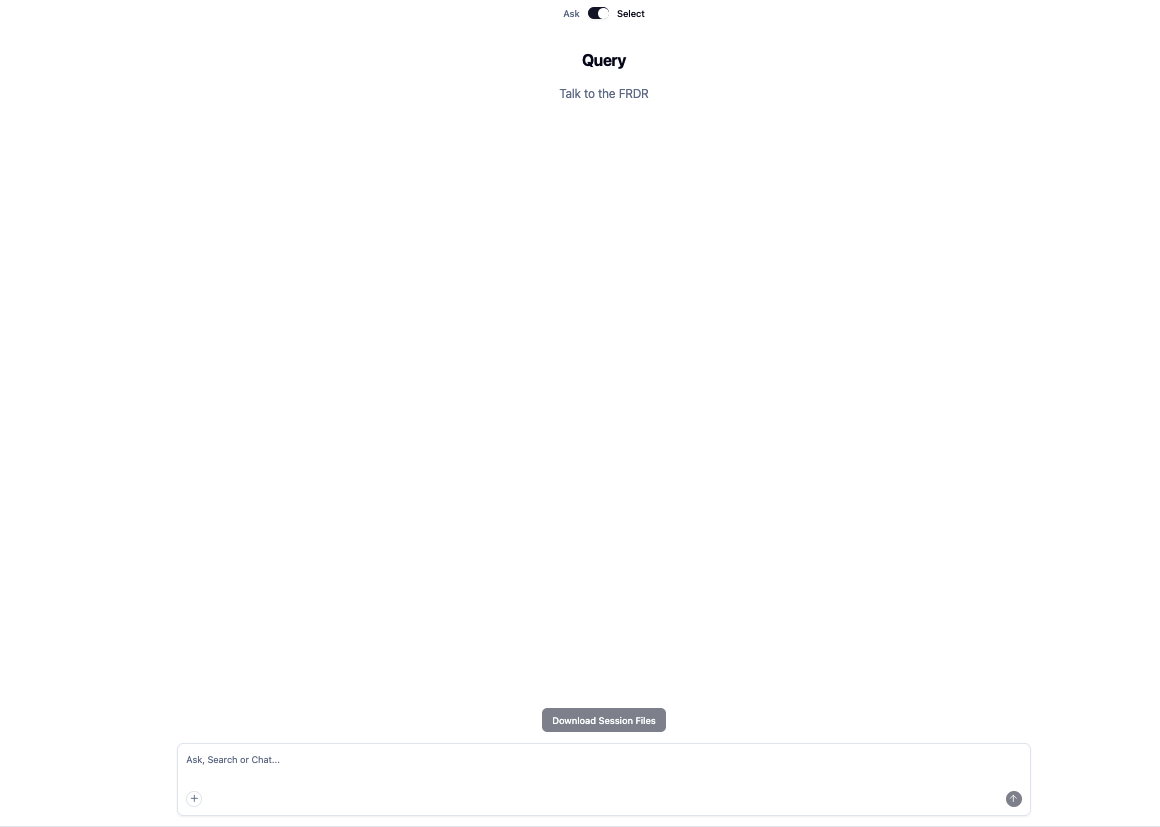
\includegraphics[width=0.95\textwidth]{QueryPage.png}
\caption{Query: use Select when you need tables and downloads.}
\label{fig:query}
\end{figure}

\subsection{Workflow D: See how much data exists and list sessions}
\label{wf:inventory}

\begin{enumerate}
  \item Open \textbf{Inventory} (\emph{Data Inventory}).
  \item Quick start: press \textbf{Show full inventory} or \textbf{Unoperated rats only}, \emph{or} expand filters on the left (drugs, file types, brain and apparatus fields, session type).
  \item Press \textbf{Apply}. The main area shows session count, counts by file type, and a bar chart.
  \item To see rows: press \textbf{View sessions (up to 500)}. A table appears when loading finishes.
  \item To download files for listed sessions: use \textbf{Download Session Files} in the left panel (only after step~4 produced a non-empty table). Pick formats and confirm as in Workflow~C.
  \item Press \textbf{Clear} when you want to reset filters and results.
\end{enumerate}

Use the small \textbf{(i)} icons on cards for short definitions (for example what counts as one \emph{session}).

\subsection{Workflow E: Inspect one session in depth}
\label{wf:toolbox}

\begin{enumerate}
  \item Open \textbf{ToolBox} (\emph{Analysis Toolbox}).
  \item In \emph{Search or select a session\ldots}, type part of an ID; pick a row from the dropdown.
  \item Press \textbf{Load Session}. Wait until loading finishes.
  \item Read \textbf{Session Info}, then \textbf{Data Points} (scroll the table). View the image if shown, and the \textbf{interactive path} diagram.
  \item Read the three summary cards: distance, total checks, average check time (shown as log$_{10}$ seconds). If distance says it is not available, press \textbf{Generate Distance?} once.
\end{enumerate}

If the app says the session is not supported, try another ID or confirm with your team.

\begin{figure}[ht]
\centering
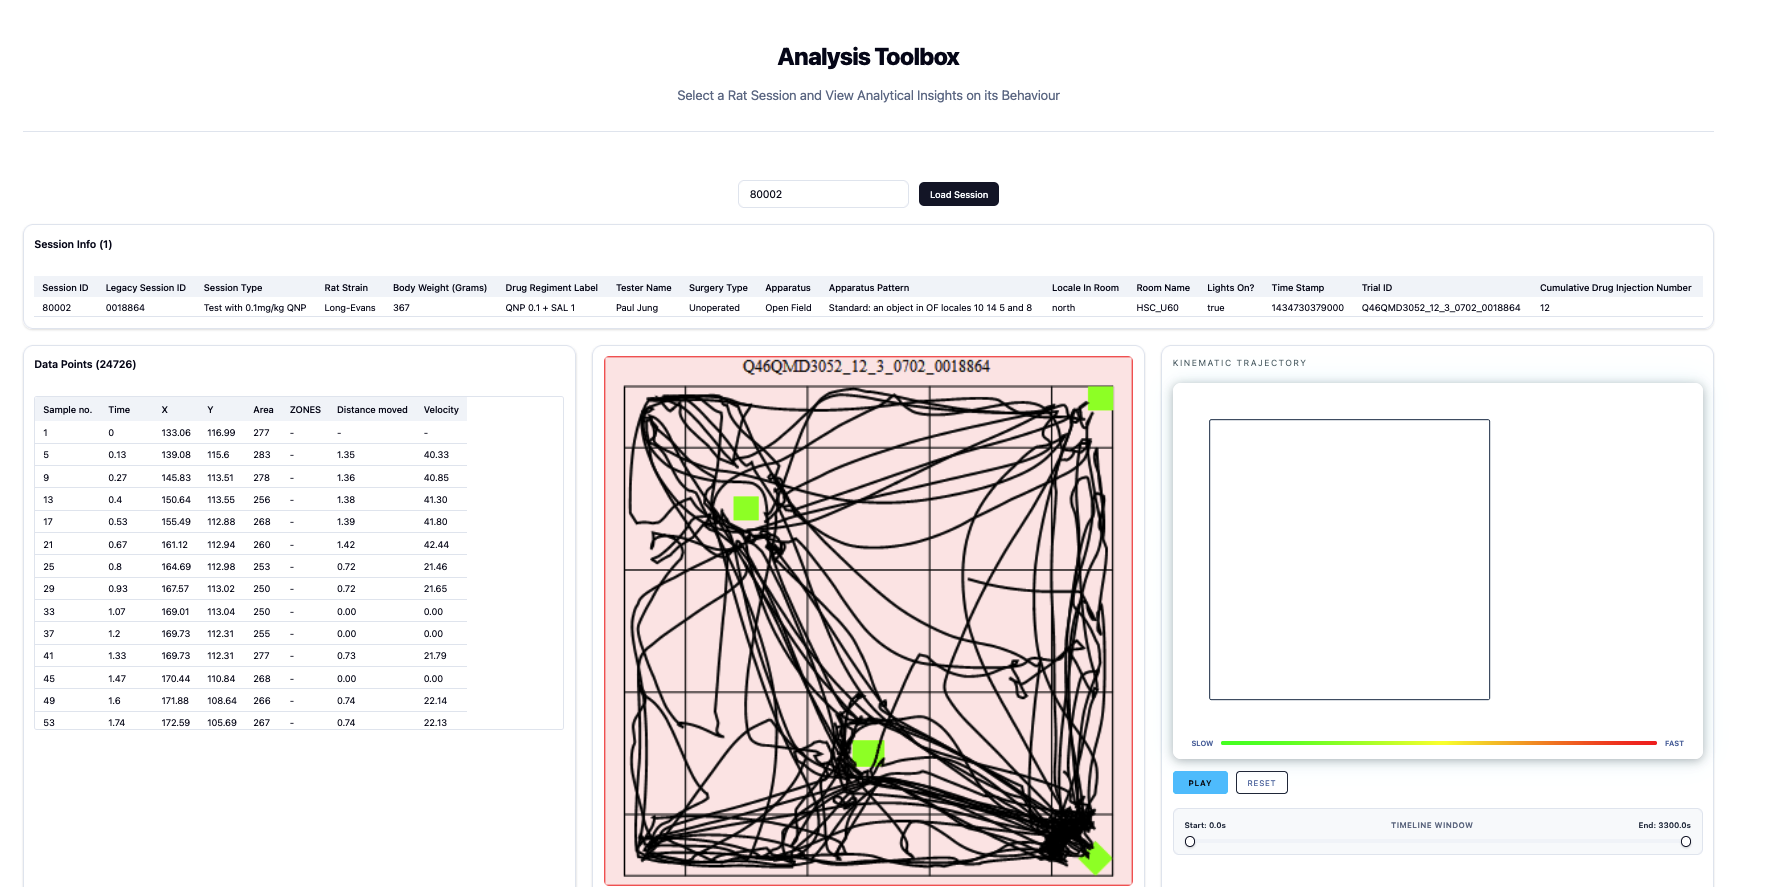
\includegraphics[width=0.95\textwidth]{ToolBoxPage.png}
\caption{ToolBox: follow search $\rightarrow$ Load $\rightarrow$ tables and metrics.}
\label{fig:toolbox}
\end{figure}

\subsection{Workflow F: Build a bar chart, heatmap, or line chart}
\label{wf:charts}

\begin{enumerate}
  \item Click \textbf{Visualizations}. You see a gallery of tiles; press \textbf{Open} on \textbf{Bar Chart} or \textbf{Heatmap}.
  \item For a \textbf{bar chart}: choose \textbf{X-Axis (Group By)} and \textbf{Y-Axis}; the chart updates from your choices.
  \item For a \textbf{heatmap}: choose two dimensions and a \textbf{metric} for colour.
\end{enumerate}

\textbf{Line chart} (trends over time) is \textbf{not} listed on the gallery page. If your group uses it, ask for the direct link or bookmark it when someone shares it. On that page, choose \textbf{X-Axis (Time Period)} and a \textbf{Y-Axis} metric.

\begin{figure}[ht]
\centering
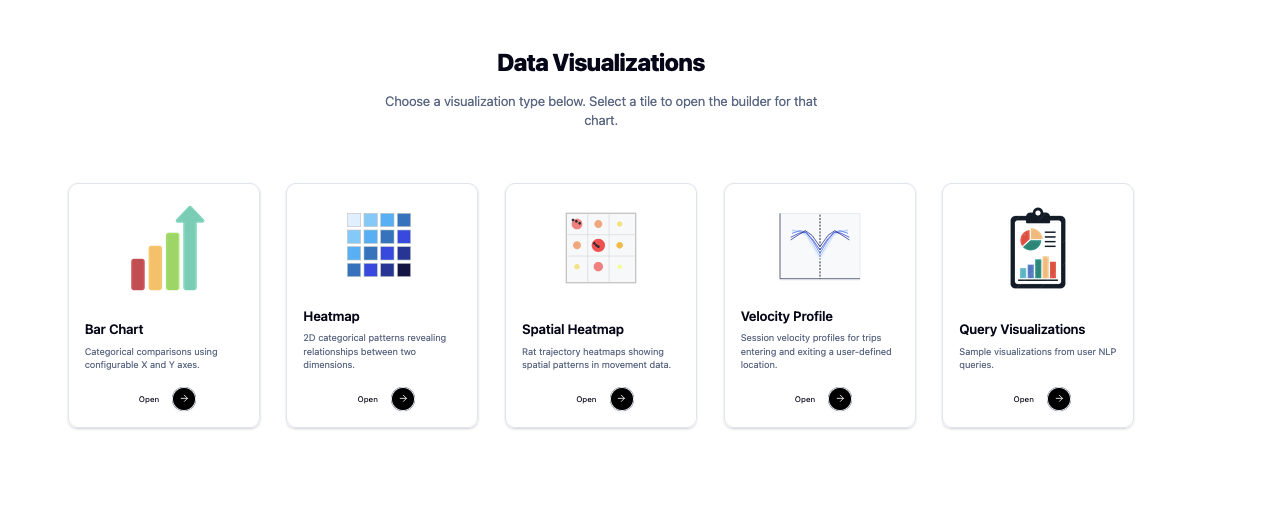
\includegraphics[width=0.95\textwidth]{Visualizations.png}
\caption{Visualizations: choose a tool, then Open.}
\label{fig:visualizations}
\end{figure}

\subsection{Workflow G: Map where animals spent time (spatial heatmap)}
\label{wf:spatial}

\begin{enumerate}
  \item From \textbf{Visualizations}, open \textbf{Spatial Heatmap}.
  \item Under \textbf{Sessions}, tick one or more IDs; use \textbf{Clear All} to reset. Unsupported sessions are listed in a message.
  \item Set \textbf{Bin size (cm)} and the \textbf{metric}: \emph{Entries (Visits)} or \emph{Time Spent}.
  \item Optionally set \textbf{Fixed scale max} so colours stay comparable across sessions.
  \item Optionally define a \textbf{home base}: enter the four corners in centimetres, press \textbf{Set Home Base}; the page can show time in that region as a percentage. Use \textbf{Clear} to remove it.
  \item Move the mouse over the map to inspect bins. Use \textbf{Export Data to CSV} or \textbf{Export Map to PNG} to save your work.
\end{enumerate}

\subsection{Workflow H: Speed into and out of a zone (velocity profile)}
\label{wf:velocity}

\begin{enumerate}
  \item From \textbf{Visualizations}, open \textbf{Velocity Profile}.
  \item \textbf{Select session} with the search field (same idea as ToolBox).
  \item \textbf{Define zone:} enter centre $X$, $Y$, and \textbf{Radius}. If you need coordinates, load the session in \textbf{ToolBox} first and read values from the data or plot.
  \item Set \textbf{Max frames per side} and \textbf{Min trip frames} (short segments are treated as lingering and skipped).
  \item Choose \textbf{Colouring}: \emph{Temporal gradient} or \emph{Time-slice highlight} (then use the slider under the chart when applicable).
  \item Press \textbf{Generate}. Read the summary tiles and the chart. If nothing appears, try a larger radius or a smaller minimum trip length.
\end{enumerate}

\subsection{Workflow I: Compare groups on standard measures (dashboards)}
\label{wf:dashboard}

\begin{enumerate}
  \item From \textbf{Visualizations}, open \textbf{Query Visualizations}.
  \item Read the title and description for the selected layout.
  \item Open the \textbf{Graph Set} menu and choose a format (for example Tucci-style snapshot bars or Ballester-style lines across injections).
  \item Scan the grid of panels (checking frequency, check length, recurrence, stops before returning, rest duration, and related measures depending on the set).
  \item Hover points or bars for mean, error, and sample size when offered. If one panel fails, others may still load---read any warning at the top.
\end{enumerate}

\subsection{Workflow J: Get help or contact the team}
\label{wf:about}

\begin{enumerate}
  \item Click the \textbf{info} icon (\textbf{About}).
  \item Expand FAQ items for purpose, audience, data types, and downloads.
  \item If you still need detail, use the button to go to \textbf{Query} and ask there, or use \textbf{GitHub} from the header for technical issues.
\end{enumerate}

\section{Reference}
\label{sec:reference}

\subsection{ZIP downloads (Query and Inventory)}
\label{ref:zip}

Bulk downloads are one ZIP per job. You choose which types to include:

\begin{description}[style=nextline, font=\normalfont\bfseries]
  \item[CSV] Spreadsheet-friendly tables.
  \item[EWB] Behavioural workflow files for the research pipeline.
  \item[JPG] Still images.
  \item[MPG] Videos.
  \item[GIF] Short animations.
\end{description}

Spatial heatmap \textbf{Export to CSV/PNG} is separate from this ZIP flow.

\subsection{Glossary}
\label{sec:glossary}

\begin{description}[style=nextline, font=\normalfont\bfseries]
  \item[Ask] Chat answers without a results table or Query-page ZIP download.
  \item[Select] Mode that shows a plan, SQL, and results; required for downloads on the Query page.
  \item[FRDR] Federated Research Data Repository; mentioned on Query and in download names.
  \item[Session] One behavioural trial for one animal (see Inventory tooltips).
  \item[Graph set] A named dashboard layout on \textbf{Query Visualizations}.
  \item[Home base] A rectangle on the spatial heatmap used to measure time in a region.
\end{description}

\subsection{If something goes wrong}
\label{sec:troubleshooting}

\begin{itemize}[nosep]
  \item \textbf{Download on Query is greyed out.} Send another message in \textbf{Select} that returns a table, and make sure that message is the \textbf{last} one in the thread.
  \item \textbf{Download on Inventory is greyed out.} Run \textbf{View sessions (up to 500)} and wait for a non-empty table.
  \item \textbf{ToolBox menu does nothing or errors.} Refresh the page; if it persists, contact your administrator (the registered address may differ by host).
  \item \textbf{Empty chart.} Try other axis or metric choices.
  \item \textbf{Stuck progress bar.} Wait for the current job to finish; refresh only if it hangs a long time.
\end{itemize}

\end{document}
